\documentclass[a4paper,10pt]{article}

\usepackage[T1]{fontenc}


%\renewcommand{\rmdefault}{ppl} %Palatino
%\renewcommand{\rmdefault}{cmfib} % computer modern fibonacci 365
%\renewcommand{\rmdefault}{\sfdefault} default serifenlos
\usepackage{ae}
\renewcommand{\familydefault}{phv} % Helvetica angenehm zu lesen ! 386
\usepackage{graphicx}

% Silbentrennung
\usepackage[english,ngerman]{babel}

% PDF
%LaTeX erzeugt mit dem hyperref-Paket interaktive PDF-Dateien mit Bookmarks
\usepackage{color}
\usepackage[colorlinks]{hyperref}
\usepackage{my} % modifizierte Ueberschriften
%\usepackage{avant}
%\usepackage{mathptmx}

%empfohlen aber gehen leider nicht:
%\usepackage{microtype} Optischer Randausgleich besserer Rand
%\usepackage{mparhack}


%Einstellungen der Seitenränder
% \usepackage[left=3cm,right=3cm,top=3cm,bottom=3cm,includeheadfoot]{geometry}

%Umlaute ermöglichen
\usepackage[latin1]{inputenc}
\usepackage{tabularx} % Seite 259 im Latex Buch, ist extrem cool !!
\newcolumntype{Y}{>{\small\raggedright\arraybackslash}X}


%Kopf- und Fußzeile
\usepackage{fancyhdr}
\pagestyle{fancy}
\fancyhf{}

%Kopfzeile mittig
\fancyhead[C]{\nouppercase{\leftmark}}
%Linie oben
\renewcommand{\headrulewidth}{0.5pt}

%Fußzeile mittig
\fancyfoot[C]{\thepage}
%Linie unten
\renewcommand{\footrulewidth}{0.5pt}





\begin{document}

{\sc Die Schriftart small caps (Kapit"alchen).}
{\sf Die Schriftart sans serif (serifenlos).}

\tableofcontents
\newpage

\section{Parser}

The first set is very interesting for a top down parser. The parser compares the actual token with the first-sets symbol and takes decisions between alternatives. To guarantee that the decision between two alternatives is correct, the first set of the alternatives must be disjunctive. 

% TODO umschreiben (ANFANG)
%We defined the first-sets and follow-sets to check that we can really achieve that a lookahead of one symbol is sufficient.

%The first set very interesting for a top down analysis, because it determines the progress of the analysis.
%The first set of a node contains all token, by which the parser will be guided to the node.

%If the actual text isn't matched by one of the token of the first set, an other node will be chosen, namely the node with the first set that contains a token, which matches. If there is no such alternative the parsing is stopped with an error message. To guarantee that the decision between alternatives is definite, the first sets of the alternatives must be disjunctive, i.e.: there may not be a token contained in two alternative first sets. 

% TODO umschreiben (ENDE)

\subsection{First Sets}

% use packages: array
\begin{tabular}{p{4cm}l}
	S & First(S) \\ \hline
	& \\
	program & package\_declaration package\_import  \\
	package\_declaration & "package" \\
	package\_import & "import" \\
	class\_declaration & "public" \\
	class\_block & method\_declaration datatype\_declaration \\
	method\_declaration & "public" \\
	datatype\_declaration & "static" datatype\_decsriptor \\
	method\_call & identifier \\
	datatype\_assignment & identifier \\
	body\_block & while\_statement if\_statement return\_statement datatype\_declaration identifier (method\_call datatype\_assignment) \\
	while\_statement & "while" \\
	if\_statement & "if" \\
	return\_statement & "return" \\
	datatype\_decsriptor & datatype \\
	datatype & primitive object \\
	primitive & "int" "boolean" "char" \\
	object & String identifier \\
	identifier & letter \\
	selector & "." "[" \\
	condition & expression \\
	expression & term \\
	term & factor \\
	factor & value \\
	value & identifier datatype not\_value TODO \\
	integer & "-" digit\_non\_zero \\
	char & "'"\\
	boolean & "true" "false" \\
	string & """ \\
	digit & digit\_non\_zero digit\_zero \\
	digit\_non\_zero & 1 2 3 4 5 6 7 8 9 \\
	digit\_zero & 0 \\
\end{tabular}


\begin{figure}
	\begin{center}
	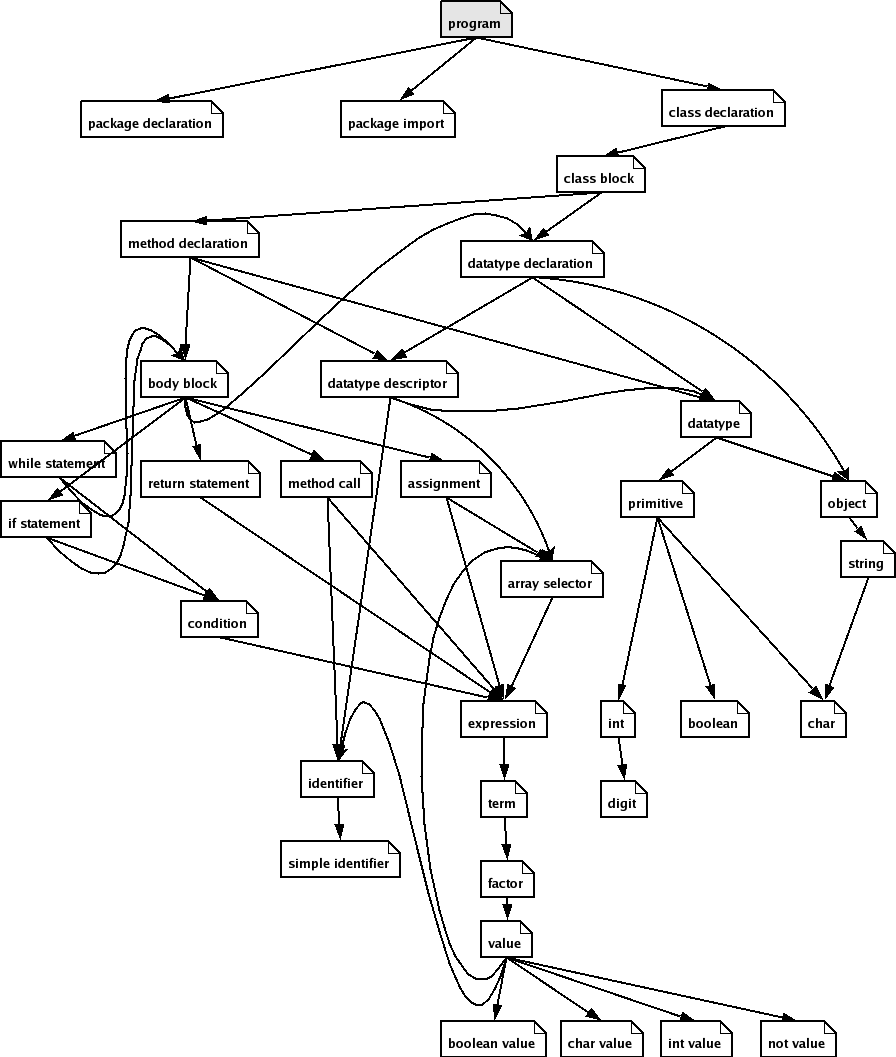
\includegraphics[scale=0.4]{Diagram_Small.png}
% Diagram_Small.eps: 300dpi, width=10.83cm, height=12.67cm, bb=0 0 1279 1497 ,bb=0 0 1279 1497
% width=15cm,height=15cm
	
	\label{dep_diagram}
	\caption {Dependencies representation of parsing procedures (simplified).}
	\end{center}
\end{figure}





\end{document}
